% Generated by thesis/ch7/exp2/networks.py -- do not edit by hand.
\begin{sidewaysfigure}
  \centering
  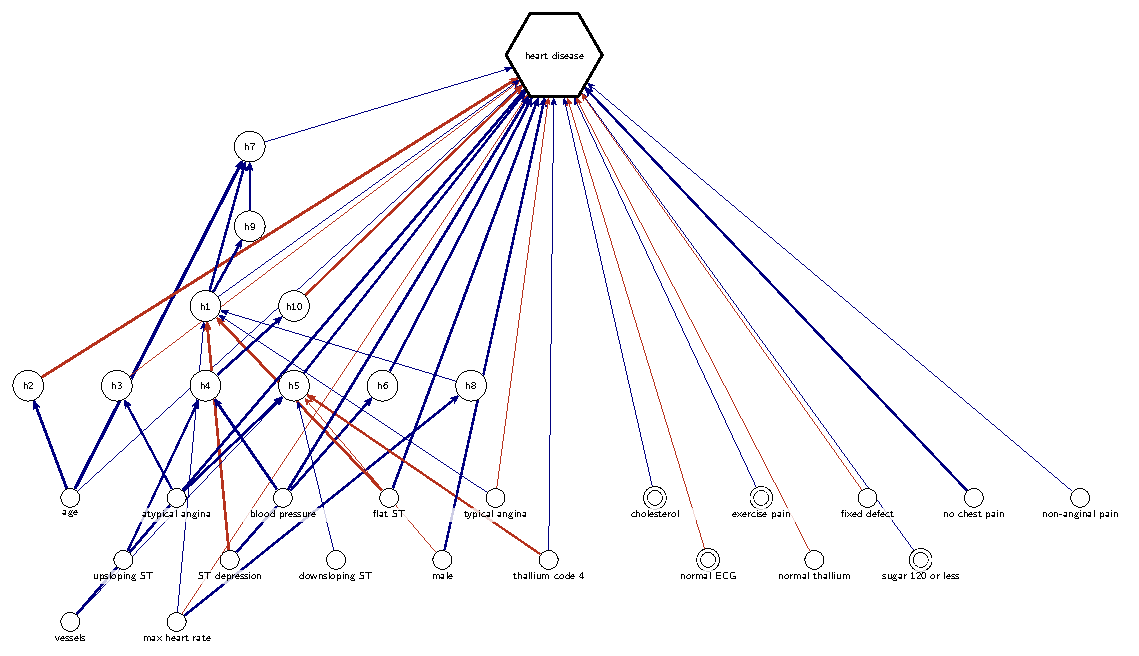
\includegraphics[width=\textheight,height=0.78\textwidth,keepaspectratio]{figures/exp2/networks/heart100-s3-raw}
  \caption{Heart-100, seed 3 (heart100-s3): the network as trained, before any explanation, in full. Inputs at the bottom (every input column its own node), hidden units by depth, the output at the top; 20 of 26 input columns are connected, with 10 hidden units and 45 enabled connections. Blue: positive weight (raises the score); red: negative weight (lowers it); thicker: larger weight. Orange outline and up arrow: raises the final prediction; teal and down arrow: lowers it; grey and double arrow: depends. Not used (no connection; 6 columns): female, sugar above 120, ST-T abnormal ECG, LVH on ECG, no exercise pain and reversible defect.}
  \label{fig:exp2-net-heart100-s3-raw}
\end{sidewaysfigure}
